\documentclass[12pt,twoside,vi]{mitthesis}
\usepackage[T1]{fontenc} % font encoding
\usepackage[numbers]{natbib}
\usepackage{graphicx}
\PassOptionsToPackage{hyphens}{url}\usepackage{hyperref}
\usepackage{color}
\newcommand{\wip}[1]{{\color{red} To do...}}
% \newcommand{\wip}[1]{{\color{red} #1}}
\begin{document}
\title{Git-Based Platform for Distributed Learning Communities}
\author{Vahid Fazel-Rezai}
\department{Department of Electrical Engineering and Computer Science}
\degree{Master of Engineering in Computer Science and Engineering}
\degreemonth{June}
\degreeyear{2018}
\thesisdate{May 25, 2018}
\supervisor{Philipp Schmidt}{Research Scientist, Director Media Lab Learning Initiative}
\chairman{Katrina LaCurts}{Chairman, Department Committee on Graduate Theses}
\maketitle
\cleardoublepage
\setcounter{savepage}{\thepage}
\begin{abstractpage}
Instructors use software called learning management systems to administer online courses. Traditionally these digital platforms mimic physical classrooms, but new technology opens up potential for interactions not previously possible. In this thesis, we build a learning management system on top of git to create a learning environment that encourages collaboration and exploration. We discuss how it was designed following established learning principles, the technical implementation, and the results of a pilot online class, with 80 learners lasting 6 weeks, as part of the Refugee Learning Accelerator. The platform architecture used in this study can be replicated and reused for other online courses with similar goals.
\end{abstractpage}
\cleardoublepage
\section*{Acknowledgments}
\wip{Acknowledgments...}

\tableofcontents

\newpage
\listoffigures

\newpage
\listoftables

\chapter{Introduction}

New education technology, enabled by the Internet, has allowed learners to connect with their instructors and with each other digitally. Pieces of software known as learning management systems take the experience of a classroom online, giving remote learners more access to education and enriching their learning experiences with a variety of technology.

In this thesis I employ git, a version control technology initially created for collaboration among software developers, as the foundation for an experimental learning platform. The decentralized nature of git can be utilized to expand interactions beyond replicating that which is found in traditional course. New interactions can be designed to balances the benefits of a collective learning experience with those of independent open-ended projects. In this study, I develop a prototype of such a platform and examine the results of a pilot run in an online course. As a result of this work, I hope to contribute to lowering the barrier of entry to administer an online course using a git-based learning platform. The design decisions map out an architecture that can be built upon in future courses. 

The following sections outlines the approach taken towards this study. Chapters 2 and 3 cover the established theory and other similar projects that were taken as guidance in designing the new platform. Chapter 4 steps through the design and implementation of the platform; section 4.3 is the only section in this thesis that assumes a technical background. Finally, results of a pilot run of using the platform in an online course are presented in chapter 5. 

\section{Refugee Learning Accelerator}

The development of a git-based learning platform is part of a larger project called the Refugee Learning Accelerator (RLA). RLA is a program run by the Learning Initiative, a group of the MIT Media Lab. The goal of the program is to gather and support technologists from the Middle East to work on education tools for refugee learners. 

The program ran in three phases from fall of 2017 through spring of 2018. First, interested candidates applied as teams through an open application. Around 100 participants were selected for the first phase of the program, which consisted of a 6-week online course during November and December of 2018. Every two weeks of the course, a new technology was introduced and teams were challenged to design, and ideally build a prototype for, an education solution using that technology. Webinars held throughout the 6 weeks helped participants learn about the technologies. Additionally, teams received constructive feedback every week, once at the midpoint and once at the end of each challenge. The topics chosen for the online course were chatbots, human centered design, and AR/VR. A description of each challenge is included in Appendix A.

The second phase of the program brought 14 selected teams together for a week-long, in-person workshop in Amman, Jordan. There, teams forged their project ideas through rapid iterations of feedback and field observation. One important aspect of the workshop was also the building of a supportive community, where members encourage one another to pursue their projects and help in connecting each other to resources.

Following the workshop, teams worked independently to bring their projects to fruition in partnership with local NGOs and with the continued support of the RLA community.~\cite{rla}

RLA is the product of the collective effort by members of the Learning Initiative and others passionate about finding creative ways to nurture learning, including the motivated participants, many of whom were working on their projects meanwhile also taking on a full-time load at work or as a student. The team of instructors included researchers and students from MIT and other affiliated experts. Mentors and speakers from all backgrounds donated their time to assisting teams through the webinars and at the workshop. The development of a learning platform was just one component in the operation of creating and executing the RLA program. 

While one of my goals in building the platform was certainly to support the online course of RLA, I also hoped to explore the possibilities in its design. In this way, the online course of RLA served also as a pilot run for the platform in order to evaluate its utility and shortcomings. 

\section{Methodology}

Ultimately the research question I hope to answer in this thesis is: how can git be adapted to support effective online learning?

This can be covered in three parts:
\begin{itemize}
	\item First, I turn to established theory on digital learning pedagogy and principles to guide the characteristics and ultimately define interactions of the platform. In particular, I derive these interactions from first principles of learning and target learning outcomes rather than by attempting to move traditional classroom interactions online.
	\item Second, I implement a technical platform that supports these interactions. The bulk of this work is done before the pilot course, but also includes the technical operation of the course. As much as possible, I rely on third-party software to increase reliability, reproducibility, and familiarity. Creating a learning platform from scratch is beyond the scope of this work.
	\item Third, I use the pilot run to evaluate not only how these interactions work in the manifested platform, but also how well they work. In order to gather feedback, I conducted an anonymous survey among participants in the online course. This consisted of a form send by email, the questions of which are included in Appendix B. Responses to the survey as well as anecdotal evaluation are reported in Chapter 5.
\end{itemize}

The code and course content are all freely available online for use in future iterations of such research.~\cite{rla}

\chapter{Background}

Educational theory and pedagogy is a vast field and far outdates the advent of online education. Here we briefly touch on frameworks that went into consideration for this thesis. 

\section{Traditional Learning Platforms}

An online platform to support learning is not a new concept. A learning management system (LMS) is a tool that helps instructors supervise an online course, and popular commercial LMSs exist such as Blackboard, Moodle, and Canvas. 

A traditional LMS platform typically provides features including tracking learner grades, file management for assignments and corresponding submissions, and communication mechanisms for instructor announcements or learner questions. These features are often more convenient duplicates of the same in-person interactions of traditional classrooms. Furthermore, LMS usually don’t fully encompass the activities of a class, leaving the core of the learning for classroom instruction or learner self-study. 

Of note, the issue of learner collaboration, which is often a component of more creative, project-based assignments, is often not properly addressed in traditional LMS platforms. This intersection of collaboration and technology is instead known as computer-supported collaborative work (CSCW), and families of tools exist to support online collaboration. Learners thus would have to take to these external tools to collaborate, depending on the particular assignment.

\section{Foundational Theory}

We begin with the assumption that humans have innate desire and ability to pursue their interests, and the role of the learning environment is to foster the right conditions. To break down this idea, we rely on 



\wip{Assuming SDT (autonomy, relevance, competence), which explains why humans have an innate desire to do things and have individualized passions, we use the 4P's to achieve learning outcomes (reason ------ design ----, work collaboratively.... mitch reference)

We had several goals in mind when deciding how to craft the online course, which can be summarized in four principles: 
Projects. 
Peers. 
Passion. 
Play. 
We believe learners do best when they are engaged in th

These principles largely rely on students being drivers of their own learning. 

We turn to self-determination theory (SDT) as a model with which to understand learners’ motivation. SDT [citation needed]

Self-determination theory: autonomy, competence, relatedness. Hence, we prioritize these in designing features of the platform.
}

\section{Pedagogical tensions}

\wip{overall course vs community.........

4 tensions content vs connection, individual pathway vs shared experience, solitary vs team, projects vs puzzles

for each tension, there are benefits to both sides, it's a matter of balancing the two

pedagogy and platform are closely linked but not causully linked

mastery->feedback, community}

\chapter{Related Work}

We set out to develop a new platform to address 

\section{Overview of git}

A specific technology used for online collaboration, particularly in software engineering, is git. Created in 2005 by Linus Torvalds as a tool to support the development of the Linux kernel, git allows users to each have a local copy of a set of files and sync between their copy and a central server in a coordinated fashion. Git is also a version control system, hence allowing users to backtrack changes or split into multiple branches of work from the same starting state. [git]

Git is used as a command line tool, in which users type text commands to perform the desired git actions. In addition, there are graphical interfaces available which serve as a wrapper and aid for users who prefer not to use the command line. Overall, git is considered a powerful collaboration tool, but involves an upfront investment to learn its operations.

\section{Communities of practice}

Use of group chats such as gitter and mattermost to complement projects

\section{Other uses of git}

While git was initially created for and has been largely relied on by the software development community, its use has spread to other knowledge workers.

An example of applying git to a traditional use case is cookbooks: a service called Fork the Cookbook exists in which users can fork, or copy, an existing recipe and tweak it to make it their own. This creates a collaborative and decentralized platform for sharing cooking recipes.~\cite{forkthecookbook}

Example applications include recipes, legislation, datasets, general CMS, etc.

\section{Existing git-based learning systems}

\chapter{Platform Development}

\section{Design}

In this section we lay out the high-level design for the RLA course. The git-based platform is developed as just one of the components of this course, but is always intended to be applicable outside the context of RLA to other future courses.

\subsection{Balancing tensions}

We also aimed to foster a community that would extend into the later phases of the Accelerator. 

Finally, we rely on good software development practices and use popular tools where possible.

Communication. Communication lays the groundwork for the type of community formed. We aim to have instructors clearly communicate how to use the platform and be able to guide students throughout the course. We would like to allow natural and structured opportunities to ask questions and give feedback. General course information should be readily accessible to students.

Permissions. We will have to decide how to control authority to perform actions and visibility of content. On one hand, we believe that the platform should be as open as possible. This would allow students the opportunity to pursue their curiosities, to learn from each other’s work, and to feel that they have a complete understanding of the platform. On the other hand, we would like to prevent either intentional or accidental actions that may destroy or hinder other participants’ work. We also anticipate that sensitive topics would not be expressed without a private way of doing so and thus would like to allow for that.

\subsection{Suitability of git}

While git was not designed as a learning platform, we found in it suitable qualities. Here we discuss the benefits of git as a tool for fostering positive educational interactions.

As a version control system, the currency is units of work rather than final deliverables. It is oriented around building larger projects through a series of work. Git gives learners room to play, since branches can be made to explore new ideas and unsuccessful changes can be easily reverted. It is also very much designed for collaborating with peers. After all, its raison detre is to be able to build upon each others’ work without conflict. Documenting everyone’s work openly and allowing collaboration creates a shared space from which a community could form, just as many have in the open source world. It gives flexibility in what tools people can use for their work, since all file types are supported. Finally, because git is already widely-used, its kinks have been worked out and help material is readily available online, making it easier for new adopters.

As discussed in the previous section, git can also be adapted as the underlying mechanism of a content management system. As a versioning system, git enables publishing new content, updates, and revisions in a fashion that can be distributed. Popular git hosting websites such as Github and GitLab have built-in support for Markdown-formatted files and support and static web pages.

\subsection{Platform architecture}

The details of the design were chosen to support the needs of RLA’s weekly cycle. In each week of the cycle, content is released at the beginning and learners worked towards a particular milestone by the end of the week. Throughout the week learners can collaborate and participate in seminars.

To achieve these requirements, there are four interactions that the core git-based platform needs to support:
\begin{itemize}
\item \textbf{Onboarding.} We want learners to be able to register for the course as easily as possible, yet still provide basic information to introduce themselves to the rest of the learner community. 
\item \textbf{Content distribution.} New material posted at the beginning of the week includes a description of the week’s challenge and targeted milestones. In addition, relevant resources relevant for the week are gathered and provided for learners’ reference. This content may also sometimes include skeleton code or template documents in which learners can report their progress. These pieces of content require the additional ability of being pulled into learners’ working directories.
\item \textbf{Submission.} At the end of the week, learners need a mechanism to put together a package representing the state of their work on which to receive feedback. We also encourage learners to use these submissions as a resource to learn from other learners’ approach to the challenge.
\item \textbf{Feedback.} We believe frequent personalized feedback can be helpful to learners and also cultivates a culture of collaboration. Hence we’d like our platform to provide an interface where a reviewer can easily peruse a learner’s work and leave comments. Note that this process is similar in structure to code review used in software engineering, so we can utilize similar features in the git hosting service.
\end{itemize}

In addition to managing the course content, we also want to support a few forms of communication that empower learners:
\begin{itemize}
\item For seminars, we need a way to broadcast video to learners. Additionally, we would like to engage learners to drive the conversation according to their passions and have face-time with their peers.
\item For technical support and other miscellaneous discussion, we would like to have an open, real-time, group chat. In particular, the group aspect will expose the entire community to conversations as appropriate so that everyone feels included and in-the-know.
\item For showcasing teams' work, especially to parties outside the course, it would be ideal to have a static website summarizing the challenges and the progress coming out of the course. Anyone could then share the link and in this way feel ownership over their work.
\end{itemize}

\section{Third-party Software}

\subsection{Git hosting service}

In order to have a group of distributed learners participate in the course using git, we needed to have an server accessible by the Internet running git where the content would be hosted. We looked at two of the most popular git hosting services, Github and GitLab. Both offer a SaaS model where they host git on their servers and simply provide an interface, as well as a self-hosted version where they provide the software but leave running a server to the customer.

We compared options the two in terms of features, styles, and technical performance.

The two options had very similar sets of features. Github has organizations, teams, repositories, and pull requests, while GitLab has groups, subgroups, projects, and merge requests. Both expose a webhook for git commits, allow in-browser editing of files, and can serve hosted files as static websites. Both offer free or discounted private repositories/projects for educational uses. On a few points GitLab had additional features, such as being able to request to join a group and being able to trigger scripts that run before serving static websites.

Many software companies use Github to host either all their code or even just their open source projects, and as a result a Github profile feels very much like a professional portfolio. We wanted to make sure learners are comfortable experimenting and making mistakes, and took into consideration that some may feel less inclined to do so if the work would permanently be associated with their professional portfolio. 

Finally, we took into consideration the technical reliability of each option. We found that GitLab’s SaaS offering, GitLab.com, was often slow to load. For both, a self-hosted instance would include considerable setup and costs to run a server, but would allow customizations such as the domain name. Finally, though both are welcoming homes to open source projects, Gitlab has made the web platform itself open source, whereas Github’s is not.

For our course, we ended up opting for GitLab, and chose to mitigate performance issues by using a self-hosted instance of the free tier. However, it would certainly be possible to adapt our approach for either GitLab or Github, in the both SaaS and self-hosted models.

\subsection{Chat service}

To allow the development of a community, we wanted to make communication among learners as well as between learners and instructors as open as possible. GitLab alone, with commit messages and comments on merge requests, did not offer as fluid of a setting as we wanted. We decided to augment GitLab with a team-based chat service where learners could communicate in real time.

We looked at existing cloud messaging services including Slack, Gitter, and Mattermost, all of which have a very similar design. They provide open channels where any user can join and chat, as well as messaging between users and in private groups for more direct communication. We hoped to use these spaces as a forum for discussing ideas, asking each other for help, and even just to meet other learners.

From our options we chose to run a self-hosted instance of Mattermost, largely due to our choice of self-hosted GitLab. Mattermost and GitLab have a built-in integration for authentication and backend configuration. Mattermost is also open source, continuing in our spirit of relying on open source tools.

\subsection{Server infrastructure}

\wip{reliance on other software (letsencrypt, nginx, python and javascript, bash)}

\section{Technical Implementation}

\wip{In this section we outline the initial implementation of the platform. We assume a technical background, in particular familiarity with Internet architecture and git.
6.1 Server configuration
DigitalOcean droplet https://www.digitalocean.com/community/tutorials/how-to-install-and-configure-gitlab-on-ubuntu-16-04 
GitLab [built in for DO]
NameCheap domain and networking
nginx customization
Lets encrypt
6.2 Repo architecture
Brief overview of possibilities
Step by step description of how it all worked
6.3 Scripts
As much as possible, git-related operations of the platform were automated to ease the burden on the instructors. 
Onboarding membership request poller
Onboarding group creation
Health check with email notifications
Create subtrees
Create merge request
Merge
Analyze progress}


\chapter{Results of RLA Pilot}

For six weeks in October and November of 2017, the approximately 80 learners participated in an online course using a git-based learning platform as the first phase of the RLA program. Following the course, an optional survey was conducted, the questions of which are included in the appendix. In this section we report the experience, results, and feedback we observed in the course and survey responses.

\section{User Experience}

\begin{figure}[H]
\centering
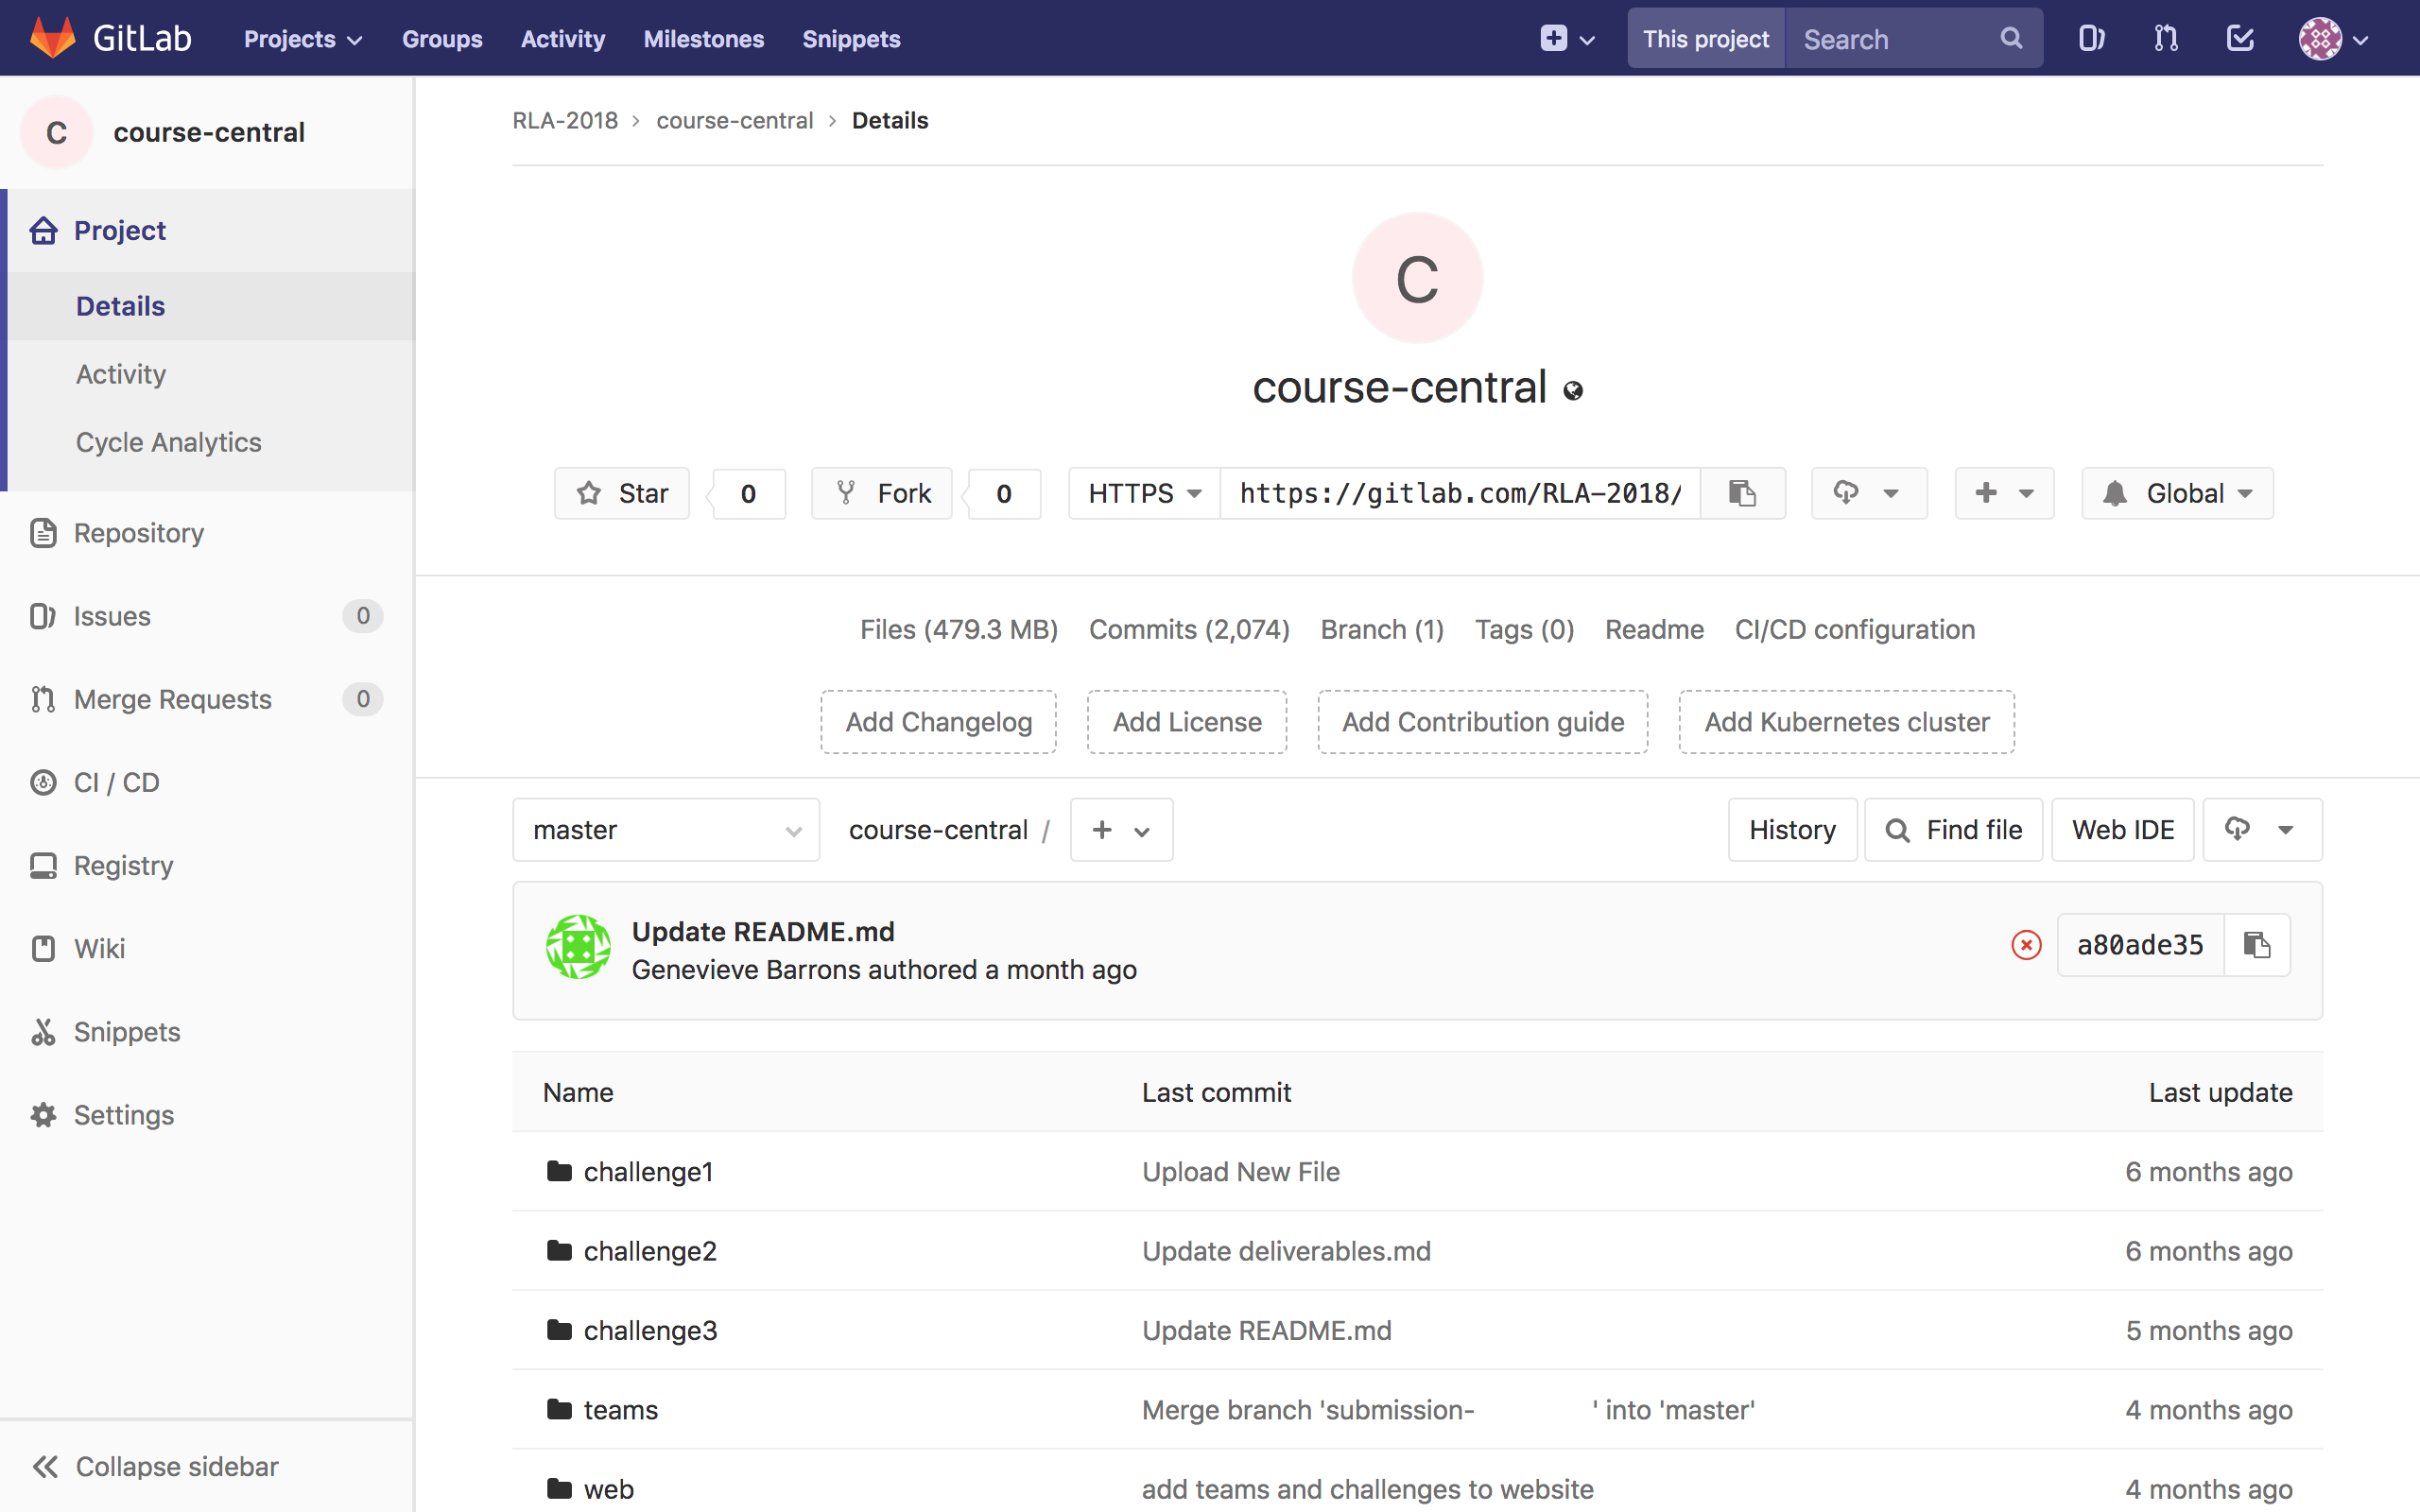
\includegraphics[scale=0.3]{fig-course-central.png}
\caption{The \texttt{course-central} repository.}
\end{figure}

\wip{Frame around tensions, for each broad set of interactions go over "what did it look like", "how did it work", and "how well did it work"}

\chapter{Conclusion}

\wip{narrative summary of thesis, an honest set of personal takeaways (from which reader can judge whether to replicate work) and feeligns about future work}

\appendix

\chapter{RLA Challenge Descriptions}

The online course was divided into three challenges, each of which had two sets of deliverables (one for each week). Here we provide brief descriptions of these. More information as well as various resources related to the topics of each challenge is available online.~\cite{rla} All content was developed by members of the MIT Media Lab Learning Initiative unless otherwise noted.

\begin{enumerate}
\item \textbf{Challenge 1 - chatbots:} How might we use chatbots to support refugee learners inside or outside of the classroom? 
\begin{itemize}
\item Describe your concept for a chatbot in one or two paragraphs. Use visuals (mockups, diagrams) if possible. It is important to be as specific as possible while mapping out the scope of the project as this will greatly influence implementation and the tools to use. Answer the following questions:
\begin{itemize}
\item What problem/ challenge will the chatbot solve? 
\item How will the chatbot solve it? 
\item Who is the primary user and how will the chatbot engage the user?
\item What activity does the chatbot facilitate that would not otherwise be possible? 
\item What challenges do you expect to encounter?
\end{itemize}
\item Demonstrate how your chatbot works. Videos, screenshots or images are encouraged. Add a short description and answer the following questions: 
\begin{itemize}
\item How did you build it? (Platform and technology)
\item What challenges did you face?
\item What aspect of the chatbot do you like best? 
\item What would you different in the future? 
\item Please also add a link to your code!
\end{itemize}
\end{itemize}
\item \textbf{Challenge 2 - human centered design:} How might we use everyday technologies as learning tools?
\begin{itemize}
\item Make an initial prototype. Questions to answer:
\begin{itemize}
\item What solution are you testing? (and why did you choose it?)
\item Submit your prototype (use photos, video, diagrams etc.)
\item Describe the prototype and why you chose this prototyping method. 
\item What did you learn during the prototyping process?
\item Who are your intended users for testing?
\end{itemize}
\item Test it with users. Questions to answer:
\begin{itemize}
\item How did you select your test users? 
\item What was the setting of the test? 
\item What were the main points of feedback you received (share a summary)? 
\item What changes would make to your idea/project based on the feedback?
\item What parts of the Human Centered Design process were new to you?
\item What parts of the Human Centered Design process seemed most useful to you?
\end{itemize}
\end{itemize}
\item \textbf{Challenge 3 - augmented reality (AR):} How might we use Augmented Realtiy (AR) to support refugee language learning outside the classroom?
\begin{itemize}
\item Describe your concept for how low fidelity Augmented Reality could be used to support language learning in one or two paragraphs. Use visuals (mockups, diagrams) if possible. It is important to be as specific as possible while mapping out the scope of the project as this will greatly influence implementation and the tools to use. Answer the following questions:
\begin{itemize}
\item What problem/challenge will the AR experience solve? 
\item How will the AR experience solve it? 
\item Who is the primary user and how will the AR experience engage the user?
\item What hardware does the user need? Is this realistic in the refugee context? 
\item What activity does the AR experience facilitate that would not otherwise be possible? 
\item What challenges do you expect to encounter? 
\end{itemize}
\item Demonstrate how your AR experience works. Videos, screenshots or images are encouraged. Add a short description and answer the following questions: 
\begin{itemize}
\item How did you build it? (Platform and technology)
\item What challenges did you face?
\item What aspect of the AR experience do you like best? 
\item What would you different in the future? 
\item Please also add a link to your code!
\end{itemize}
\end{itemize}
\end{enumerate}

\chapter{RLA Online Course Survey}

The following questions were sent in an email to participants to gather feedback and evaluate how well the platform worked. The survey was anonymous and asked for consent for responses to be used in this research study. A total of 11 participants chose to respond.

\begin{enumerate}
\item Git
\begin{itemize}
\item How much had you used git before the course?
\item To what extent did you learn git during the course?
\item How useful would you say knowledge of git was for collaborating with your team?
\end{itemize}
\item Course materials
\begin{itemize}
\item Did you have any difficulty accessing course materials? If so, what were they?
\item Did you find the course materials helpful in working on your projects? If so, which materials were most helpful?
\end{itemize}
\item Signing up
\begin{itemize}
\item Did everyone on your team submit their own initial sign up on GitLab?
\item How many people on your team used GitLab after the initial sign up? Was there a reason some did not?
\item Did you find it useful to have a list of participants in the course?
\end{itemize}
\item Submission
\begin{itemize}
\item Would you have preferred an automatic, continuous submission (as opposed to your work being snapshot at a set time)?
\item Did you run into any issues in submitting your work? If so, what were they?
\item Were you able to see other team's submitted work? If so, did you find that useful?
\end{itemize}
\item Seminars
\begin{itemize}
\item What were your favorite and least favorite features of the Unhangout platform for seminars?
\item Did you find the seminars useful in ideating for your projects? If so, were any seminars particularly useful?
\item Did you find the seminars useful for the technical side of your projects? If so, were any particularly useful?
\end{itemize}
\item Team
\begin{itemize}
\item How was the technical work distributed among your team?
\item Was your team physically located in the same place?
\end{itemize}
\end{enumerate}

\clearpage
\newpage
\begin{singlespace}
\nocite{*}
\bibliography{sources} 
\bibliographystyle{apa}
\end{singlespace}
\end{document}


write chapter 2

write chapter 3

write chapter 4

spin up new server

write chapter 5

write chapter 6

read proposal and copy relevant text

proofread

